\setcounter{ExampleCounter}{1}
\begin{center}

\includegraphics[width=0.8\textwidth]{gambling}
\end{center}
In 1654, a French writer who called himself Chevalier de M\'er\'e (it must have sounded better than his real name, Antoine Gombaud), wrote a letter to two mathematicians, Blaise Pascal and Pierre de Fermat.  He had a question about a game of chance, and the mathematicians leaped at the gambler's challenge.  Between the two of them, they began to develop the theory of probability, and gambling was never the same again.

One of the problems that Pascal and Fermat considered was related to flipping a coin repeatedly.  If you flip a coin once, what's the probability that it comes up heads?  Since there are two possibilities, and each is equally likely, the answer is 1/2 or 50\%.  Now, what if you flip a coin twice?  How many heads could you get?  Here are all the possibilities:
\begin{center}
HH \hspace{0.5in} HT \hspace{0.5in} TH \hspace{0.5in} TT
\end{center}
Notice that you could get a total of 2 heads (1 out of 4), 1 head (2 out of 4), or 0 heads (1 out of 4).  We can graph this:
\begin{center}
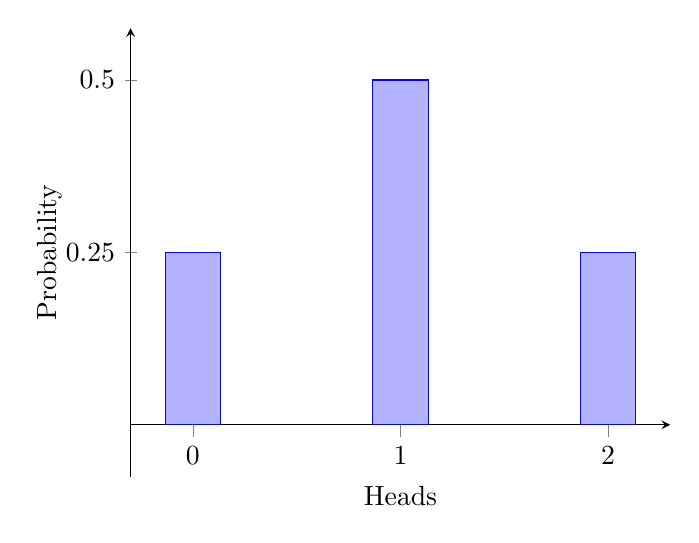
\begin{tikzpicture}
\begin{axis}[
	x tick label style={
		/pgf/number format/1000 sep=},
    axis lines=middle,
	ylabel={Probability},
	xlabel={Heads},
	x label style={at={(axis description cs:0.5,0)},anchor=north},
    y label style={at={(axis description cs:-0.11,.5)},rotate=90,anchor=south},
    xtick={0,1,2,3},
	xticklabels={,0,1,2},
	ytick={0,0.25,0.5,0.75},
	yticklabels={0,0.25,0.5,0.75},
	enlargelimits=0.15,
	%legend style={at={(0.5,-0.1)},
	%anchor=north,legend columns=-1},
	ybar,
	bar width=20pt,
	ymin=0,
	ymax=0.5,
	%nodes near coords,
	%nodes near coords style={
	%	/pgf/number format/.cd,fixed zerofill,precision=1},
	%nodes near coords align={vertical},
]
\addplot 
	coordinates {(1,0.25) (2,0.5)
		 (3,0.25)};
\end{axis}
\end{tikzpicture}
\end{center}

It turns out that, as the number of coin flips increases, an interesting pattern emerges.  However, the results always have the following two features present:
\begin{enumerate}
\item The probabilities are symmetric (notice above how the probability of 2 heads and 0 heads are equal).
\item The highest probability occurs at the center, and decreases from there out to the extremes.
\end{enumerate}
The second feature makes sense, because it would be really unusual to get a long unbroken string of heads or tails; a mixture is more common, and the likeliest result would be to get an even number of each.
\pagebreak

Here are the graphs for larger numbers of trials (flipping the coin 10 or 20 times):
\begin{center}
\begin{tabular}{c c}
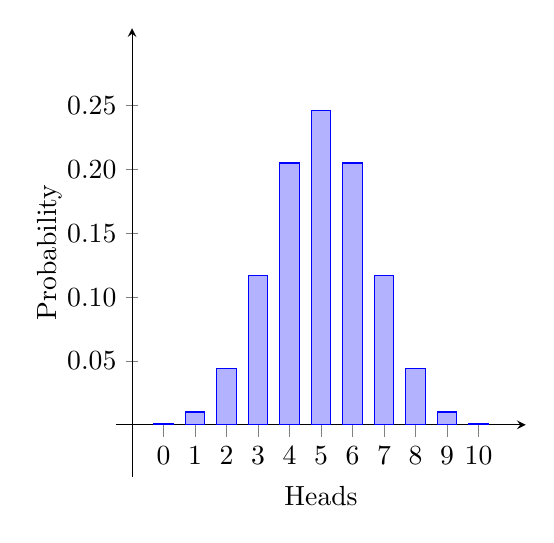
\begin{tikzpicture}
\begin{axis}[
	x tick label style={
		/pgf/number format/1000 sep=},
    axis lines=middle,
	ylabel={Probability},
	xlabel={Heads},
	x label style={at={(axis description cs:0.5,0)},anchor=north},
    y label style={at={(axis description cs:-0.11,.5)},rotate=90,anchor=south},
	xtick={0,1,2,3,4,5,6,7,8,9,10,11},
	xticklabels={,0,1,2,3,4,5,6,7,8,9,10},
	ytick={0,0.05,0.10,0.15,0.20,0.25},
	yticklabels={0,0.05,0.10,0.15,0.20,0.25},
	enlargelimits=0.15,
	%legend style={at={(0.5,-0.1)},
	%anchor=north,legend columns=-1},
	ybar,
	bar width=7pt,
	ymin=0,
	ymax=0.27,
	x=0.4cm,
	%nodes near coords,
	%nodes near coords style={
	%	/pgf/number format/.cd,fixed zerofill,precision=1},
	%nodes near coords align={vertical},
]
\addplot 
	coordinates {(1,0.001) (2,0.01) (3,0.044) (4,0.117) (5,0.205)
		(6,0.246) (7,0.205) (8,0.117) (9,0.044) (10,0.01) (11,0.001)};
\end{axis}
\end{tikzpicture}
&
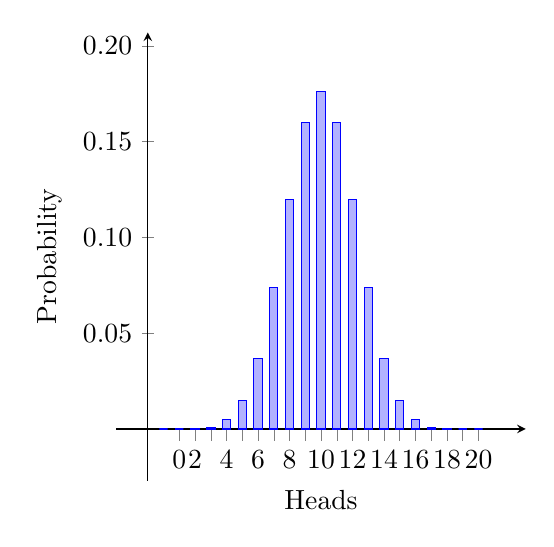
\begin{tikzpicture}
\begin{axis}[
	x tick label style={
		/pgf/number format/1000 sep=},
    axis lines=middle,
	ylabel={Probability},
	xlabel={Heads},
	x label style={at={(axis description cs:0.5,0)},anchor=north},
    y label style={at={(axis description cs:-0.11,.5)},rotate=90,anchor=south},
	xtick={0,2,3,4,5,6,7,8,9,10,11,12,13,14,15,16,17,18,19,20,21},
	xticklabels={,0,2,,4,,6,,8,,10,,12,,14,,16,,18,,20,},
	ytick={0,0.05,0.10,0.15,0.20,0.25},
	yticklabels={0,0.05,0.10,0.15,0.20,0.25},
	enlargelimits=0.15,
	%legend style={at={(0.5,-0.1)},
	%anchor=north,legend columns=-1},
	ybar,
	bar width=3pt,
	ymin=0,
	ymax=0.18,
	x=0.2cm,
	%nodes near coords,
	%nodes near coords style={
	%	/pgf/number format/.cd,fixed zerofill,precision=1},
	%nodes near coords align={vertical},
]
\addplot 
	coordinates {(1,0) (2,0) (3,0.0002) (4,0.001) (5,0.005)
		(6,0.015) (7,0.037) (8,0.074) (9,0.12) (10,0.16) (11,0.176)
		(12,0.16) (13,0.12) (14,0.074) (15,0.037) (16,0.015)
		(17,0.005) (18,0.001) (19,0.0002) (20,0) (21,0)};
\end{axis}
\end{tikzpicture}
\end{tabular}
\end{center}

The shape of this graph starts to look smoother and smoother for higher numbers, but it always keeps this particular shape:
\begin{center}
\begin{tikzpicture}
\begin{axis}[
  no markers, domain=-4:4, samples=100,
  axis lines*=none,
  hide y axis,
  every axis y label/.style={at=(current axis.above origin),anchor=south},
  every axis x label/.style={at=(current axis.right of origin),anchor=west},
  height=5cm, width=12cm,
  xtick=\empty, ytick=\empty,
  enlargelimits=false, clip=false, %axis on top,
  %grid = major
  ]
  \addplot [very thick,cyan!50!black] {gauss(0,0.5)};
\end{axis}
\end{tikzpicture}
\end{center}

Here's the surprising part: this curve starts to pop up over and over again.  For instance, the North Carolina public school system released the average SAT score for each high school in the state.  The results are shown in the histogram below.
\begin{center}
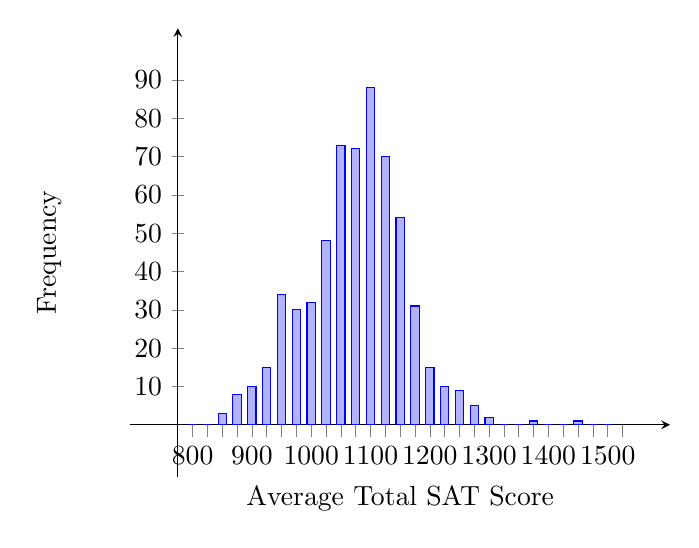
\begin{tikzpicture}
\begin{axis}[
	x tick label style={
		/pgf/number format/1000 sep=},
    axis lines=middle,
	ylabel={Frequency},
	xlabel={Average Total SAT Score},
	x label style={at={(axis description cs:0.5,0)},anchor=north},
    y label style={at={(axis description cs:-0.11,.5)},rotate=90,anchor=south},
	xtick={0,1,...,30},
	xticklabels={,800,,,,900,,,,1000,,,,1100,,,,1200,,,,1300,,,,1400,,,,1500},
	ytick={0,10,...,90},
	yticklabels={0,10,...,90},
	enlargelimits=0.15,
	%legend style={at={(0.5,-0.1)},
	%anchor=north,legend columns=-1},
	ybar,
	bar width=3pt,
	ymin=0,
	ymax=90,
	%nodes near coords,
	%nodes near coords style={
	%	/pgf/number format/.cd,fixed zerofill,precision=1},
	%nodes near coords align={vertical},
]
\addplot 
	coordinates {(1,0) (2,0) (3,3) (4,8) (5,10)
		(6,15) (7,34) (8,30) (9,32) (10,48) (11,73)
		(12,72) (13,88) (14,70) (15,54) (16,31)
		(17,15) (18,10) (19,9) (20,5) (21,2)
		(22,0) (23,0) (24,1) (25,0) (26,0) (27,1)
		(28,0) (29,0)};
\end{axis}
\end{tikzpicture}
\end{center}

In fact, almost any measurement of natural phenomena starts to exhibit this familiar pattern.  If you measure people's height, shoe size, ear length, or IQ, or the amount of milk that a cow produces, or how long a natural pregnancy lasts, you'll see the results follow this same pattern: there's a value that's the most common, and the further you get from that value, the less common the result.  It's actually more specific than that, and there's a particular mathematical pattern underlying all of this.
\pagebreak

It didn't take long for mathematicians to notice this pattern, and they gave this special curve several names: it is often called the \emph{Gaussian curve} after \marginnote{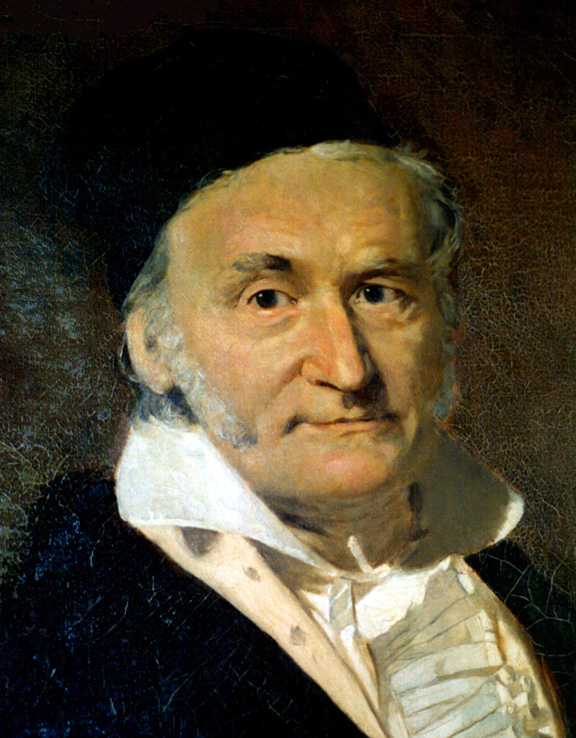
\includegraphics[height=1.0in]{Gauss}\\ \emph{C.F. Gauss}}Carl Friedrich Gauss, one of the most prolific mathematicians of all time.  It is also known as the \textbf{normal curve}\footnote{The term \emph{normal curve} was popularized by the great statistician Karl Pearson, who said this in 1920:
\begin{quote}
Many years ago [in 1893] I called the Laplace-Gaussian curve the \emph{normal} curve, which name, while it avoids the international question of priority, has the disadvantage of leading people to believe that all other distributions of frequency are in one sense or another \emph{abnormal}.
\end{quote}} or the \textbf{normal distribution}, and sometimes the term \emph{bell curve} is used in reference to its shape, how it looks similar to a bell.

\subsection{Different Bell Curves}
If you look back at the comparison between flipping a coin 10 times and 20 times, you can see that the curve, while it has the same overall form, has a different specific shape in each case: one is shorter and wider, and the other is taller and narrower.

In other words, we can observe that different normal curves have different amounts of \emph{spread}.  Because of that, it may not surprise you to learn that we can describe this spread using one of its measures that we discussed earlier in this chapter: the \emph{standard deviation}.

Also, if you look closer at those two side-by-side bar charts, you'll notice that the center occurs at different locations: in the experiment with 10 coin flips, the center is at 5, and the center is at 10 for the other.  It turns out, again with little surprise, that we can describe this center using the \emph{mean}.

\begin{formula}{Normal Curve Parameters}
Every normal curve is determined by two values: its center and spread.  Specifically, the center is defined by the \textbf{mean}, and the spread is defined by the \textbf{standard deviation}.\\

Knowing these two values tells us everything we need to know about a normal curve; they completely define its shape.
\end{formula}

Here are a few examples of different normal curves:
\begin{center}
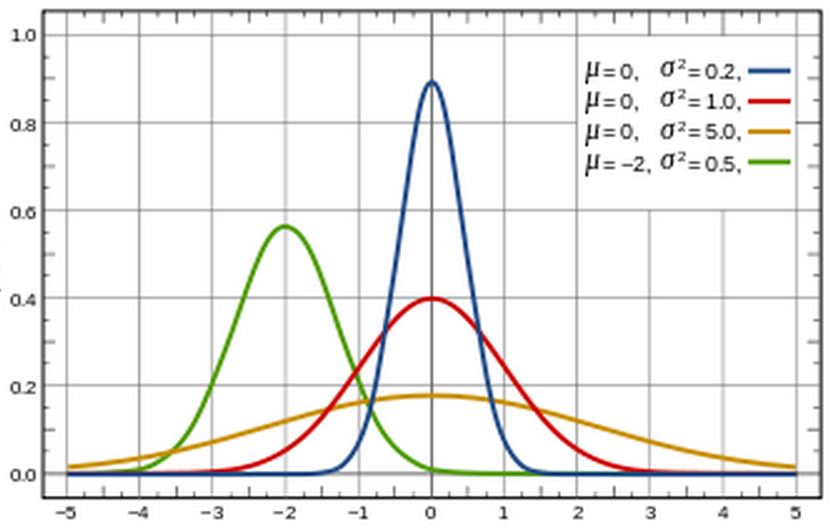
\includegraphics[height=2.5in]{MultNorm}
\end{center}

Notice how three of them have the same mean; they are centered at the same point.  They all have different standard deviations; the one with the smallest standard deviation is the narrowest (and thus the tallest), and the one with the largest standard deviation is the most spread out (and thus the shortest).

\subsection{The Empirical Rule}
The beauty of the normal distribution is that there is a predictable pattern for how likely a certain value is.  For instance, in the example of the NC SAT scores, we could predict how likely it is for a particular school's average score to be between 900 and 1000.  Or if we knew the mean and standard deviation for IQ scores, we could tell approximately how many people have an IQ over 120.
\pagebreak
\text{}
\vfill

To do this, we'll use what's called the \textbf{Empirical Rule}, which is a simplified version of a much larger concept, but it's enough for us to work with.  The Empirical Rule predicts what percentage of the data will fall within one step, two steps, or three steps of the center (mean), where the step is the size of the standard deviation.
\vfill

\begin{proc}{The Empirical Rule}

Approximately 68\% of the data is within \textbf{one} standard deviation of the mean.\\

Approximately 95\% of the data is within \textbf{two} standard deviations of the mean. \\

Approximately 99.7\% of the data is within \textbf{three} standard deviations of the mean.

\begin{center}
\begin{tikzpicture}
\begin{axis}[
  no markers, domain=-4:4, samples=100,
  axis lines*=none, xlabel=$x$,
  hide y axis,
  every axis y label/.style={at=(current axis.above origin),anchor=south},
  every axis x label/.style={at=(current axis.right of origin),anchor=west},
  height=5cm, width=12cm,
  xtick={-3,-2,-1,0,1,2,3}, ytick=\empty,
  xticklabels={$\mu-3\sigma$,$\mu-2\sigma$,$\mu-\sigma$,$\mu$,$\mu+\sigma$,$\mu+2\sigma$,$\mu+3\sigma$},
  enlargelimits=false, clip=false, %axis on top,
  grid = major
  ]
  \addplot [fill=cyan!20, draw=none, domain=-1:1] {gauss(0,1)} \closedcycle;
  \addplot [fill=yellow!20, draw=none, domain=-2:-1] {gauss(0,1)} \closedcycle;
  \addplot [fill=yellow!20, draw=none, domain=1:2] {gauss(0,1)} \closedcycle;
  \addplot [fill=green!20, draw=none, domain=-3:-2] {gauss(0,1)} \closedcycle;
  \addplot [fill=green!20, draw=none, domain=2:3] {gauss(0,1)} \closedcycle;
  \addplot [very thick,cyan!50!black] {gauss(0,1)};


\draw [yshift=2.5cm, latex-latex](axis cs:-1,0) -- node [fill=white] {68\%} (axis cs:1,0);
\draw [yshift=1.5cm, latex-latex](axis cs:-2,0) -- node [fill=white] {95\%} (axis cs:2,0);
\draw [yshift=0.5cm, latex-latex](axis cs:-3,0) -- node [fill=white] {99.7\%} (axis cs:3,0);
\end{axis}

\end{tikzpicture}
\end{center}

Note that this diagram uses $\mu$ for the population mean (as opposed to $\overline{x}$ for the sample mean) and $\sigma$ for the population standard deviation (as opposed to $s$ for the sample standard deviation).
\end{proc}
\vfill

As you can see, another name for the Empirical Rule is the ``68-95-99.7 Rule.''  Let's try an example using this rule.
\vfill

\begin{example}[https://www.youtube.com/watch?v=XcZCDQln9L0]{College Entrance Exams}
The scores on a college entrance exam are normally distributed with a mean of 52 points and a standard deviation of 11 points. About 95\% of the values lie between what two scores?

\sol
We know that 95\% of the data is within two standard deviations of the mean.\\
\begin{align*}
\textrm{Scores } &= \textrm{ mean } \pm (2)(\textrm{standard deviation})\\
&= 52 \pm (2)(11)\\
&= 52 \pm 22\\
&= \boxed{(30, 74)}
\end{align*}

Hence, 95\% of the values fall between a score of 30 and a score of 74.
\end{example}
\vfill
\text{}
\vfill
\pagebreak

\begin{example}[https://www.youtube.com/watch?v=cTRr0B5Cp8k]{The Intelligence Quotient}
IQ is normally distributed with a mean of 100 and a standard deviation of 15. Use the Empirical Rule to the find the data that is within one, two, and three standard deviations of the mean.

\sol
\begin{center}
\begin{tikzpicture}
\begin{axis}[
  no markers, domain=-4:4, samples=100,
  axis lines*=none, xlabel=$x$,
  hide y axis,
  every axis y label/.style={at=(current axis.above origin),anchor=south},
  every axis x label/.style={at=(current axis.right of origin),anchor=west},
  height=5cm, width=12cm,
  xtick={-3,-2,-1,0,1,2,3}, ytick=\empty,
  xticklabels={55,70,85,100,115,130,145},
  enlargelimits=false, clip=false, %axis on top,
  grid = major
  ]
  \addplot [fill=cyan!20, draw=none, domain=-1:1] {gauss(0,1)} \closedcycle;
  \addplot [fill=yellow!20, draw=none, domain=-2:-1] {gauss(0,1)} \closedcycle;
  \addplot [fill=yellow!20, draw=none, domain=1:2] {gauss(0,1)} \closedcycle;
  \addplot [fill=green!20, draw=none, domain=-3:-2] {gauss(0,1)} \closedcycle;
  \addplot [fill=green!20, draw=none, domain=2:3] {gauss(0,1)} \closedcycle;
  \addplot [very thick,cyan!50!black] {gauss(0,1)};


\draw [yshift=2.5cm, latex-latex](axis cs:-1,0) -- node [fill=white] {68\%} (axis cs:1,0);
\draw [yshift=1.5cm, latex-latex](axis cs:-2,0) -- node [fill=white] {95\%} (axis cs:2,0);
\draw [yshift=0.5cm, latex-latex](axis cs:-3,0) -- node [fill=white] {99.7\%} (axis cs:3,0);
\end{axis}

\end{tikzpicture}
\end{center}

\begin{enumerate}
\item 68\% of the data is within one standard deviation of the mean.
\begin{align*}
\textrm{IQ } &= \textrm{ mean } \pm (1)(\textrm{standard deviation})\\
&= 100 \pm (1)(15)\\
&= \boxed{(85,115)}
\end{align*}

Thus, 68\% of people have an IQ between 85 and 115.

\item 95\% of the data is within two standard deviations of the mean.
\begin{align*}
\textrm{IQ } &= \textrm{ mean } \pm (2)(\textrm{standard deviation})\\
&= 100 \pm (2)(15)\\
&= 100 \pm 30\\
&= \boxed{(70,130)}
\end{align*}

Thus, 95\% of people have an IQ between 70 and 130.

\item 99.7\% of the data is within three standard deviations of the mean.
\begin{align*}
\textrm{IQ } &= \textrm{ mean } \pm (3)(\textrm{standard deviation})\\
&= 100 \pm (3)(15)\\
&= 100 \pm 45\\
&= \boxed{(55,145)}
\end{align*}

Thus, 99.7\% of people have an IQ between 55 and 145.
\end{enumerate}

Again, this rule gives a way to decide whether a data point is unusual or not.  An IQ of over 130 is very unusual, and an IQ of over 145 is even more so.\\

Since 99.7\% have IQs in the range from 55 to 145, only 0.3\% of people have IQs outside that range.  Since the bell curve is symmetric, half of those, or 0.15\% of people (15 people out of 1000) have IQs over 145.
\end{example}

\begin{try}
The mean height of boys 15 to 18-years old from Chile is 170 cm with a standard deviation of 6 cm. Male heights are known to be normally distributed. Using the Empirical Rule, find the range of heights that contain approximately 68\%, 95\%, and 99.7\% of the data.
\end{try}
\pagebreak
\text{}
\vfill

Let's go back to the figure from that last example:\\
\vfill

\begin{center}
\begin{tikzpicture}
\begin{axis}[
  no markers, domain=-4:4, samples=100,
  axis lines*=none, xlabel=$x$,
  hide y axis,
  every axis y label/.style={at=(current axis.above origin),anchor=south},
  every axis x label/.style={at=(current axis.right of origin),anchor=west},
  height=5cm, width=12cm,
  xtick={-3,-2,-1,0,1,2,3}, ytick=\empty,
  xticklabels={55,70,85,100,115,130,145},
  enlargelimits=false, clip=false, %axis on top,
  grid = major
  ]
  \addplot [fill=cyan!20, draw=none, domain=-1:1] {gauss(0,1)} \closedcycle;
  \addplot [fill=yellow!20, draw=none, domain=-2:-1] {gauss(0,1)} \closedcycle;
  \addplot [fill=yellow!20, draw=none, domain=1:2] {gauss(0,1)} \closedcycle;
  \addplot [fill=green!20, draw=none, domain=-3:-2] {gauss(0,1)} \closedcycle;
  \addplot [fill=green!20, draw=none, domain=2:3] {gauss(0,1)} \closedcycle;
  \addplot [very thick,cyan!50!black] {gauss(0,1)};


\draw [yshift=2.5cm, latex-latex](axis cs:-1,0) -- node [fill=white] {68\%} (axis cs:1,0);
\draw [yshift=1.5cm, latex-latex](axis cs:-2,0) -- node [fill=white] {95\%} (axis cs:2,0);
\draw [yshift=0.5cm, latex-latex](axis cs:-3,0) -- node [fill=white] {99.7\%} (axis cs:3,0);
\end{axis}

\end{tikzpicture}
\end{center}
\vfill

What if we want to find what percentage of the data falls in some other range?  Like what about the percentage of IQs that fall between 100 and 115?  Or above 85?  Between 70 and 115?\\

All of this can be done with a little clever analysis of the figure above.  We just need to divide it up into segments that are each one standard deviation (15 IQ points) wide and figure out what percentage of the data is in each slice.\\

First of all, notice that the center region (between 85 and 115) contains 68\% of the data.  Because the graph is symmetric, we can conclude that each half of that contains 34\%.\\

Next, the two yellow regions together contain $95\%-68\% = 27\%$, so each region contains half of that, or 13.5\%.  Similarly, the two green regions account for $99.7\%-95\% = 4.7\%$, so each of them contains 2.35\% of the data.  Finally, the tails outside the green account for the remaining 0.3\% of the data, so each side contains 0.15\%.\\
\vfill

\begin{center}
\begin{tikzpicture}
\begin{axis}[
  no markers, domain=-4:4, samples=100,
  axis lines*=none, xlabel=$x$,
  hide y axis,
  every axis y label/.style={at=(current axis.above origin),anchor=south},
  every axis x label/.style={at=(current axis.right of origin),anchor=west},
  height=5cm, width=12cm,
  xtick={-3,-2,-1,0,1,2,3}, ytick=\empty,
  xticklabels={55,70,85,100,115,130,145},
  enlargelimits=false, clip=false, axis on top,
  grid = major
  ]
  \addplot [fill=cyan!20, draw=none, domain=-1:1] {gauss(0,1)} \closedcycle;
  \addplot [fill=yellow!20, draw=none, domain=-2:-1] {gauss(0,1)} \closedcycle;
  \addplot [fill=yellow!20, draw=none, domain=1:2] {gauss(0,1)} \closedcycle;
  \addplot [fill=green!20, draw=none, domain=-3:-2] {gauss(0,1)} \closedcycle;
  \addplot [fill=green!20, draw=none, domain=2:3] {gauss(0,1)} \closedcycle;
  \addplot [very thick,cyan!50!black] {gauss(0,1)};

\draw [yshift=2cm,xshift=5.9cm] node {34\%};
\draw [yshift=2cm,xshift=4.6cm] node {34\%};
\draw [yshift=0.5cm,xshift=7.2cm] node {13.5\%};
\draw [yshift=0.5cm,xshift=3.3cm] node {13.5\%};
\draw [yshift=1cm,xshift=8.5cm] node {2.35\%};
\draw [yshift=1cm,xshift=2cm] node {2.35\%};
\draw [yshift=1cm,xshift=9.8cm] node {0.15\%};
\draw [yshift=1cm,xshift=0.7cm] node {0.15\%};
\draw [yshift=4cm, latex-latex](axis cs:-1,0) -- node [fill=white] {68\%} (axis cs:1,0);
\draw [yshift=5cm, latex-latex](axis cs:-2,0) -- node [fill=white] {95\%} (axis cs:2,0);
\draw [yshift=6cm, latex-latex](axis cs:-3,0) -- node [fill=white] {99.7\%} (axis cs:3,0);
\end{axis}

\end{tikzpicture}
\end{center}
\vfill

The important point is not to memorize these percentages, but rather to understand how we figured them out.  If you can follow and recreate that process, all you'll have to memorize is the 68--95--99.7 part, and you can reproduce a picture like that one in a minute or two of quick thought.  Once you can do that, you can answer questions like the following one.
\vfill
\text{}
\vfill
\pagebreak

\begin{example}[https://www.youtube.com/watch?v=E8rczzYhOL4]{Car Sales}
Suppose you know that the prices paid for cars are normally distributed with a mean of \$17,000 and a standard deviation of \$500.  Use the 68--95--99.7 Rule to find the percentage of buyers who paid
\begin{center}
\begin{tabular}{l l}
(a) between \$16,500 and \$17,500 & (b) between \$17,500 and \$18,000\\
(c) between \$16,000 and \$17,000 & (d) between \$16,500 and \$18,000\\
(e) below \$16,000 & (f) above \$18,500
\end{tabular}
\end{center}

\sol
We can use the same process that was just described to build the following diagram, using the given mean and standard deviation.
\begin{center}
\begin{tikzpicture}
\begin{axis}[
  no markers, domain=-4:4, samples=100,
  axis lines*=none, xlabel=$x$,
  hide y axis,
  every axis y label/.style={at=(current axis.above origin),anchor=south},
  every axis x label/.style={at=(current axis.right of origin),anchor=west},
  height=5cm, width=12cm,
  xtick={-3,-2,-1,0,1,2,3}, ytick=\empty,
  xticklabels={{\$15,500},{\$16,000},{\$16,500},{\$17,000},{\$17,500},{\$18,000},{\$18,500}},
  enlargelimits=false, clip=false, axis on top,
  grid = major
  ]
  \addplot [fill=cyan!20, draw=none, domain=-1:1] {gauss(0,1)} \closedcycle;
  \addplot [fill=yellow!20, draw=none, domain=-2:-1] {gauss(0,1)} \closedcycle;
  \addplot [fill=yellow!20, draw=none, domain=1:2] {gauss(0,1)} \closedcycle;
  \addplot [fill=green!20, draw=none, domain=-3:-2] {gauss(0,1)} \closedcycle;
  \addplot [fill=green!20, draw=none, domain=2:3] {gauss(0,1)} \closedcycle;
  \addplot [very thick,cyan!50!black] {gauss(0,1)};

\draw [yshift=2cm,xshift=5.9cm] node {34\%};
\draw [yshift=2cm,xshift=4.6cm] node {34\%};
\draw [yshift=0.5cm,xshift=7.2cm] node {13.5\%};
\draw [yshift=0.5cm,xshift=3.3cm] node {13.5\%};
\draw [yshift=1cm,xshift=8.5cm] node {2.35\%};
\draw [yshift=1cm,xshift=2cm] node {2.35\%};
\draw [yshift=1cm,xshift=9.8cm] node {0.15\%};
\draw [yshift=1cm,xshift=0.7cm] node {0.15\%};
\draw [yshift=4cm, latex-latex](axis cs:-1,0) -- node [fill=white] {68\%} (axis cs:1,0);
\draw [yshift=5cm, latex-latex](axis cs:-2,0) -- node [fill=white] {95\%} (axis cs:2,0);
\draw [yshift=6cm, latex-latex](axis cs:-3,0) -- node [fill=white] {99.7\%} (axis cs:3,0);
\end{axis}

\end{tikzpicture}
\end{center}

You should be able to use the figure above to reason out that
\begin{enumerate}[(a)]
\item the percentage of buyers who spent between \$16,500 and \$17,500 was 68\%.
\item the percentage of buyers who spent between \$17,500 and \$18,000 was 13.5\%.
\item the percentage of buyers who spent between \$16,000 and \$17,000 was 47.5\%.
\item the percentage of buyers who spent between \$16,500 and \$18,000 was 81.5\%.
\item the percentage of buyers who spent below \$16,000 was 2.5\%.
\item the percentage of buyers who spent above \$18,500 was 0.15\%.
\end{enumerate}
\end{example}

\begin{try}[http://www.izzomath.com/103text/stats/example4.5/story.html]
The mean height of boys 15 to 18-years old from Chile is 170 cm with a standard deviation of 6 cm. Male heights are known to be normally distributed. Using the Empirical Rule, find
\begin{enumerate}[(a)]
\item the percentage of boys with heights between 158 and 176. 
\item the percentage of boys with heights above 188.
\item the percentage of boys with heights below 164.
\end{enumerate}
\end{try}
\vfill
\pagebreak

\subsection{Z-Scores}
We've seen that the Empirical Rule is consistent no matter what the mean and standard deviation are; the proportion of the data in each section is always the same.  We can step back and describe the location of any part of the curve by specifying how many steps (standard deviations) it is to the right or left of the center.  The following graph shows this, with positive values representing steps above the mean, and negative values below.

\begin{center}
\begin{tikzpicture}
\begin{axis}[
  no markers, domain=-4:4, samples=100,
  axis lines*=none, xlabel=$x$,
  hide y axis,
  every axis y label/.style={at=(current axis.above origin),anchor=south},
  every axis x label/.style={at=(current axis.right of origin),anchor=west},
  height=5cm, width=12cm,
  xtick={-3,-2,-1,0,1,2,3}, ytick=\empty,
  xticklabels={{$-3$},{$-2$},{$-1$},{0},{1},{2},{3}},
  enlargelimits=false, clip=false, axis on top,
  grid = major
  ]
  \addplot [fill=cyan!20, draw=none, domain=-1:1] {gauss(0,1)} \closedcycle;
  \addplot [fill=yellow!20, draw=none, domain=-2:-1] {gauss(0,1)} \closedcycle;
  \addplot [fill=yellow!20, draw=none, domain=1:2] {gauss(0,1)} \closedcycle;
  \addplot [fill=green!20, draw=none, domain=-3:-2] {gauss(0,1)} \closedcycle;
  \addplot [fill=green!20, draw=none, domain=2:3] {gauss(0,1)} \closedcycle;
  \addplot [very thick,cyan!50!black] {gauss(0,1)};

\draw [yshift=2cm,xshift=5.9cm] node {34\%};
\draw [yshift=2cm,xshift=4.6cm] node {34\%};
\draw [yshift=0.5cm,xshift=7.2cm] node {13.5\%};
\draw [yshift=0.5cm,xshift=3.3cm] node {13.5\%};
\draw [yshift=1cm,xshift=8.5cm] node {2.35\%};
\draw [yshift=1cm,xshift=2cm] node {2.35\%};
\draw [yshift=1cm,xshift=9.8cm] node {0.15\%};
\draw [yshift=1cm,xshift=0.7cm] node {0.15\%};
\draw [yshift=4cm, latex-latex](axis cs:-1,0) -- node [fill=white] {68\%} (axis cs:1,0);
\draw [yshift=5cm, latex-latex](axis cs:-2,0) -- node [fill=white] {95\%} (axis cs:2,0);
\draw [yshift=6cm, latex-latex](axis cs:-3,0) -- node [fill=white] {99.7\%} (axis cs:3,0);
\end{axis}
\end{tikzpicture}
\end{center}

Because of this consistency, we will give these values ($-3$, $-2$, etc.) a special name; we will call them \textbf{z-scores}.  A z-score is simply how many standard deviations a point is above or below the mean.  For instance, in the IQ example, an IQ score of 130 would have a z-score of 2, and in the car price example, a price of \$16,000 would have a z-score of $-2$.\\

One purpose of z-scores is to put numbers on an equal footing, in terms of how unusual they are.  For instance, consider two standardized tests, the SAT and the ACT.  These tests use completely different scales for their results, so how could you compare the scores on the two?  The answer is, you can \emph{scale the results to put them on equal footing} by finding where the score on each test falls \emph{in relation to the average}.

In other words, when you get a score back for one of these tests, instead of asking ``which number is larger,'' since that's irrelevant, you'd ask, ``how many standard deviations above the mean was each score?''\\

Before we do examples, we need a quick formula for calculating z-scores: remember that $z$ will simply count the number of standard deviations above or below the mean that correspond to a particular value in the dataset.  So then, to find the z-score for a data point in a data set with a known mean and standard deviation, we just need to find its distance from the mean, and then divide that by the standard deviation to find out how many steps it will take from the mean to reach it.

\begin{formula}{Z-Scores}
If $x$ is a data value in a data set with mean $\overline{x}$ and standard deviation $s$, the $z$-score that corresponds to that data value is
\begin{align*}
\textrm{z-score } &= \dfrac{\textrm{data value } - \textrm{ mean}}{\textrm{standard deviation}}\\
\\
z &= \dfrac{x-\overline{x}}{s}
\end{align*}
\end{formula}
\pagebreak

\begin{example}[https://www.youtube.com/watch?v=DKmhYrgywMc]{Female Heights}
Female adult height is normally distributed with a mean of 65 in. and a standard deviation of 3.5 in.\\

Find the $z$-scores of the following heights:
\begin{enumerate}[(a)]
\item 58 in.
\item 71 in.
\end{enumerate}

\sol
\begin{enumerate}[(a)]
\item The $z$-score corresponding to 58 in. is
\[z=\dfrac{58-65}{3.5} = \boxed{-2}\]
\item The $z$-score corresponding to 71 in. is
\[z = \dfrac{71-65}{3.5} = \boxed{1.71}\]
\end{enumerate}
Thus, a woman at 71 in. tall is 1.71 standard deviations above the mean, while a woman at 58 in. is 2 standard deviations below the mean.\\

It should be clear that the 58 in. tall woman is more unusual, since her height is farther from the center.
\end{example}

\begin{try}
Scores on the SAT and ACT are normally distributed:
\begin{center}
\begin{tabular}{l l l}
Test & Mean & Std. Deviation\\
\hline
SAT & 500 & 100\\
ACT & 18 & 6
\end{tabular}
\end{center}
You score 550 on the SAT and 24 on the ACT.  On which test did you have a better score, relative to everyone else who took the test?
\end{try}

We can also do a bit of algebra to work in the opposite direction, if we start with a z-score.

\begin{example}[https://www.youtube.com/watch?v=qfg_DWgY3Hg]{Working Backward from Z-Scores}
Scores on an IQ test are normally distributed with a mean of 100 and a standard deviation of 15.  Find the IQ score that corresponds to each of the following $z$-scores.
\begin{enumerate}[(a)]
\item $-1.5$
\item $2.05$
\end{enumerate}

\sol
Recall that $z=\dfrac{\textrm{data value } - \textrm{ mean}}{\textrm{standard deviation}}$
\begin{enumerate}[(a)]
\item If the $z$-score is $-1.5$:
\[-1.5=\dfrac{\textrm{IQ } - 100}{15} \longrightarrow -22.5 = \textrm{IQ } - 100 \longrightarrow \textrm{IQ } = \boxed{77.5}\]
\item If the $z$-score is $2.05$:
\[2.05=\dfrac{\textrm{IQ } - 100}{15} \longrightarrow 30.75 = \textrm{IQ } - 100 \longrightarrow \textrm{IQ } = \boxed{130.75}\]
\end{enumerate}
\end{example}
\pagebreak

\subsection{The Normal Distribution and Polls}
Suppose you're tasked with conducting a straw poll to predict the victor in a close Senate race between Candidate Smith and Candidate Jones.  You randomly poll 500 people and ask them who they plan to vote for, and 52\% of them respond Smith and 48\% Jones.  Good so far, but you begin to wonder: is this really an accurate representation of the population?  You picked a good sample, but is there any way to put a number on how certain you are that your results are a valid predictor of what the population will do?

The answer is based on the Normal Distribution.  The idea is this: if we took another sample and polled them, and then another sample, and another and another, and repeated this process many times over, the results of our poll would begin to look like a normal distribution.
\begin{center}
\begin{tikzpicture}
\begin{axis}[
  no markers, domain=-4:4, samples=100,
  axis lines*=none,
  hide y axis,
  every axis y label/.style={at=(current axis.above origin),anchor=south},
  every axis x label/.style={at=(current axis.right of origin),anchor=west},
  height=3.5cm, width=8cm,
  xtick=\empty, ytick=\empty,
  enlargelimits=false, clip=false, %axis on top,
  %grid = major
  ]
  \addplot [very thick,cyan!50!black] {gauss(0,1)};
\end{axis}

\end{tikzpicture}
\end{center}

In other words, most of those polls we conducted would look similar to each other, and they would be grouped together.  There would be a few polls that would have drastically lower percentages for Smith, and a few would have drastically higher percentages--simply due to the inherent variability of a sample that we can never fully eliminate--but most of them would be clustered around the true percentage of the population that plan to vote for Smith.  In other words, the wrong polls would be rare, and the polls that are more right would be more common.

In fact, it turns out that we can specifically define this distribution as a normal distribution, which tells us that we're--for instance--95\% confident that the results we got when we took the first poll were within two standard deviations of the mean.  Now then, if we make our sample larger, it turns out that the standard deviation on this normal distribution gets smaller, so the results are more precise.

\begin{center}
\begin{tikzpicture}
\begin{axis}[
  no markers, domain=-4:4, samples=100,
  axis lines*=none,
  hide y axis,
  every axis y label/.style={at=(current axis.above origin),anchor=south},
  every axis x label/.style={at=(current axis.right of origin),anchor=west},
  height=5cm, width=12cm,
  xtick=\empty, ytick=\empty,
  enlargelimits=false, clip=false, %axis on top,
  %grid = major
  ]
  \draw [yshift=0.5cm,xshift=1.5cm] node {smaller sample};
  \draw [yshift=2.5cm,xshift=7cm] node {larger sample};
  \addplot [very thick,cyan!50!black] {gauss(0,1)};
  \addplot [very thick,cyan!50!black] {gauss(0,0.5)};
\end{axis}

\end{tikzpicture}
\end{center}

\paragraph{Margin of Error} This allows us to define something called the margin of error.  You may have seen or heard this term in the context of polls, especially political polls.  The margin of error is an inevitable part of using a sample to predict what a larger population will do, and it only depends on $n$, the size of the sample (strangely enough, it doesn't depend on the size of the population).  The larger the sample size, the smaller the margin of error will be, and thus the more precise the results of the poll will be.

\begin{formula}{Margin of Error}
If the sample size of a poll is $n$, there is at least a 95\% chance that the sample percentage lies within \[\dfrac{1}{\sqrt{n}} \times 100\%\] of the population percent.\\  

The\marginnote{\emph{writing $\times 100\%$ simply means that we convert the decimal value $1/\sqrt{n}$ to a percentage}} margin of error with a 95\% \textit{confidence level} is $\pm \dfrac{1}{\sqrt{n}} \times 100\%$.
\end{formula}

Beware, though, that you don't take for granted that the margin of error is the only thing to worry about; we've already seen that there are other sources of error, like poor sampling.  Also, we didn't even talk about other sources of bias, like self-interest or word choice.
\pagebreak

\begin{example}[https://www.youtube.com/watch?v=V3EBPVeTaFo]{Margin of Error}
What is the margin of error on a poll with a sample size of 1000 people?\\

\sol
The margin of error is 
\[\pm \dfrac{1}{\sqrt{1000}} \times 100\% = \boxed{\pm 3.16\%}\]
A margin of error of about 3\% (which is common for many political polls) corresponds to a sample size of 1000.
\end{example}

\begin{try}
What is the margin of error on a poll with a sample size of 1800 people?
\end{try}

What if we want to work backwards: can we find the sample size needed for a particular margin of error?

\begin{example}{Sample Size}
If you want a poll to have a margin of error of 2\% or less, what's the minimum sample size you should use?

\sol
Remember that the margin of error is 
\[\dfrac{1}{\sqrt{n}} \times 100\%\]

Thus, for a margin of error of 2\%:
\[2\% = \dfrac{1}{\sqrt{n}} \times 100\%\]

If we divide both sides by 100\% (i.e. convert percentages to decimals on both sides of the equation), we get
\[0.02 = \dfrac{1}{\sqrt{n}}\]

Now, since the unknown we're solving for is in the denominator, we'll multiply both sides by $\sqrt{n}$, and then divide both sides by 0.02 (it turns out this is equivalent to flipping both sides upside down):
\begin{align*}
0.02\sqrt{n} &= 1\\
\sqrt{n} &= \dfrac{1}{0.02}\\
&= 50
\end{align*}

Finally, to get rid of the square root, we simply need to square both sides:
\begin{align*}
\sqrt{n} &= 50\\
n &= 50^2\\
&= \boxed{2500}
\end{align*}

In order for a poll to have a margin of error of 2\% or less, at least 2500 people need to be polled.  Once again, the larger the sample, the smaller the margin of error.
\end{example}

\begin{try}
If you want a poll to have a margin of error of 4.5\% or less, what's the minimum sample size you should use?
\end{try}